\documentclass[12pt,a4paper]{beamer}
\usetheme{Amsterdam}
%\usecolortheme{beaver}
\usepackage[english,french]{babel}
\usepackage{graphicx}
%\usepackage[utf8]{inputenc}  
\usepackage{fontspec}
%\usepackage[T1]{fontenc}
\usepackage{amsmath}
\usepackage{amsfonts}
\usepackage{amssymb}
\usepackage{tikz}
\usepackage{listings}
\usepackage{pgfplots}
%\pgfplotsset{compat=1.14}
\pgfplotsset{compat=newest}
\usepackage{color}

\usepackage{color}
\definecolor{mygreen}{rgb}{0,0.6,0}
\definecolor{mygray}{rgb}{0.5,0.5,0.5}
\definecolor{mymauve}{rgb}{0.58,0,0.82}
\definecolor{greenfluo}{rgb}{0,255,0}
\definecolor{blueemph}{RGB}{17,59,94}

%Underline in color
\newcommand{\coloruline}[3]{\emph{\textcolor{#1}{\underline{#2\textcolor{black}{#3}}}}}

%
\setbeamertemplate{blocks}[rounded]
%\renewcommand{\insertnavigation}[1]{}
\def\insertnavigation#1{\relax}




\lstset{
  language=Java,
  commentstyle=\color{mygreen},    % comment style
  stringstyle=\color{mymauve},     % string literal style
  keywordstyle=\color{blue},       % keyword style
  basicstyle=\footnotesize        % the size of the fonts that are used for the code
}

\title{\textbf{Algorithmique avancée}}
\subtitle{Listes chaînées}
\author{Frédéric Guyomarch}
\date{2018/2019 - Semestre 3}
\institute % (optional)
{

  Université de Lille1\\
  IUT-A de Lille

}
 

 
\logo{
\includegraphics[width=5em]{figs/iutaustl}}

%Remove Figure prefix on captures
\setbeamertemplate{caption}{\raggedright\insertcaption\par}

%Remove Control bar
\beamertemplatenavigationsymbolsempty





\begin{document}

\begin{frame}
\titlepage
\end{frame}

\begin{frame}{Introduction}
Tableaux:
\begin{itemize}
\item Taille fixe (statique)
\begin{itemize}
\item Espace alloué parfois trop grand
\item Ou trop petit
\end{itemize}
\item Accès direct
\item Solution: Liste? (dynamique)
\end{itemize}

\end{frame}

\begin{frame}{Liste}
\begin{itemize}
\item Accès itératif
\item Allocation mémoire non contiguë
\item Insertion de valeur en tête
\end{itemize}
\end{frame}

\begin{frame}{TDA Liste}
\begin{itemize}
\item Type de données abstrait Liste.
\item Une structure de données qui l'implémente $\Rightarrow$
Les listes chaînées

\end{itemize}

\end{frame}

\begin{frame}{Références et valeurs}

\begin{figure}
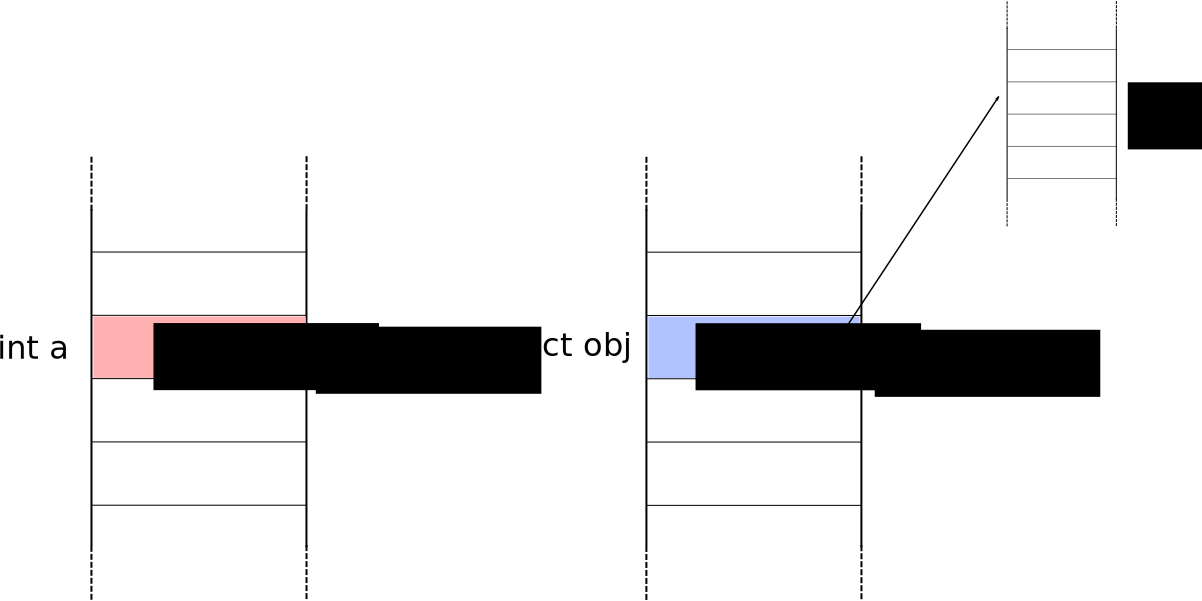
\includegraphics[scale=0.3]{figs/memoire}
\end{figure}
\end{frame}


\begin{frame}{Schéma}
\begin{figure}
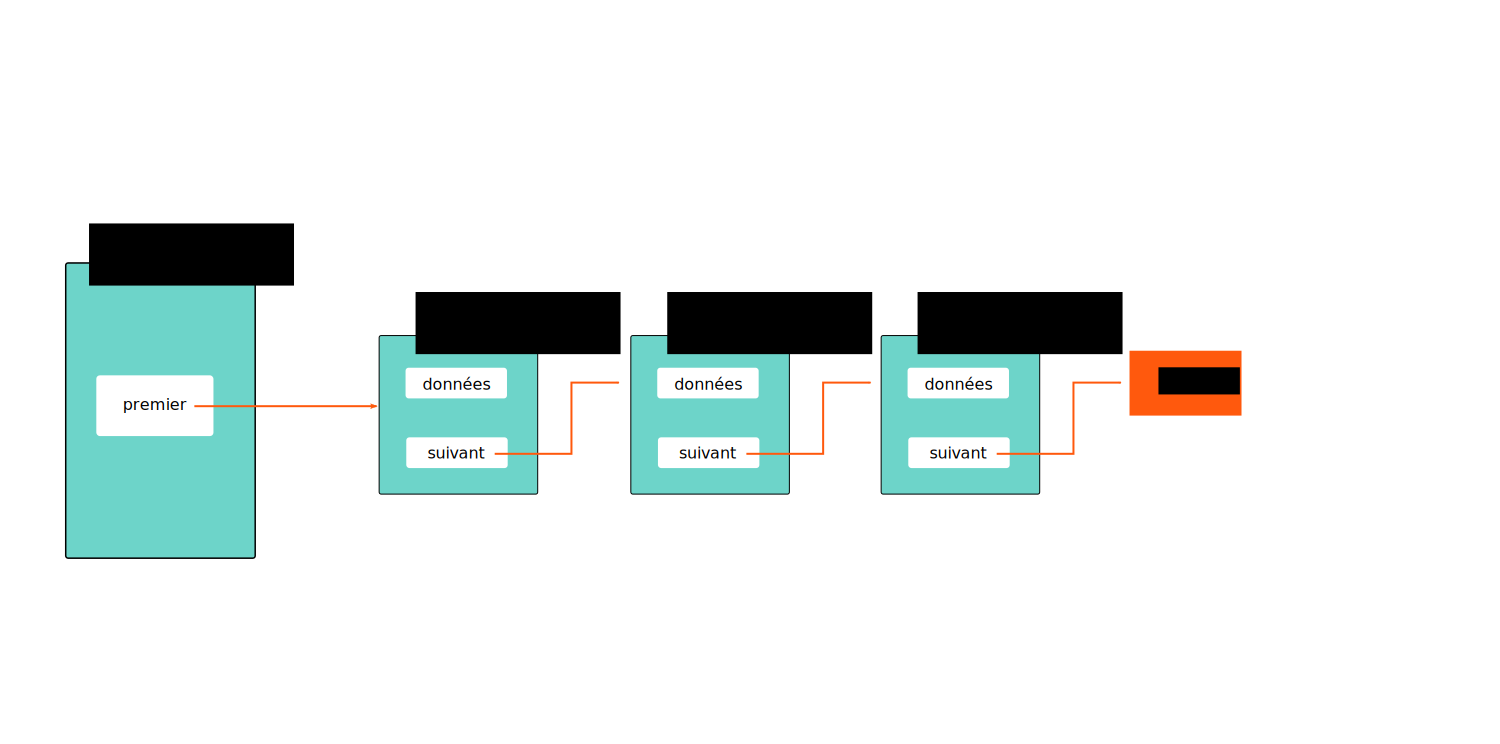
\includegraphics[scale=0.35]{figs/linked_list}
\end{figure}

\end{frame}

\begin{frame}[fragile]{et son code}
\begin{lstlisting}
class LinkedList{
  Element premier;
}

class Element{
  int iData;
  Element suivant;
}
\end{lstlisting}
\end{frame}

\begin{frame}{Insertion}
\end{frame}

\begin{frame}{Suppression}
\end{frame}

\begin{frame}{Recherche}
\end{frame}


\begin{frame}{Double-ended LinkedList}
\end{frame}



\begin{frame}{TDA Liste}
Une implémentation d'un TDA Liste: liste chaînée
\end{frame}

\begin{frame}{Pour aller plus loin...}
\begin{itemize}
\item ADT piles/files ont une taille limitée à partir d'un tableau
\item Une autre implémentation du TDA Liste: Les ArrayList
\end{itemize}
\end{frame}



\begin{frame}{Bilan}
Nous avons vu dans ce cours
\begin{itemize}
\item Une SDD dynamique
\end{itemize}
\end{frame}


\end{document}